% !TeX program = xelatex
% Fig.1 v63: redistribute height between temporal factors and shared encoding; widths unchanged.
% Native canvas 175 x 146 mm. View 0=full, 1=signal, 2=workflow, 3=compression.
% Current predecessor backed up in Figure_backup/Fig1_adaptive_shared_basis_v62.
\documentclass{article}
\providecommand{\FigOneView}{0}
\ifcase\FigOneView
  \def\PageWidth{17.5}\def\PageHeight{14.6}\def\CropX{0}\def\CropY{0}
\or
  \def\PageWidth{17.1}\def\PageHeight{2.25}\def\CropX{0.2}\def\CropY{0.1}
\or
  \def\PageWidth{6.3}\def\PageHeight{12.02}\def\CropX{0.15}\def\CropY{2.58}
\or
  \def\PageWidth{11.9}\def\PageHeight{12.02}\def\CropX{5.35}\def\CropY{2.58}
\fi
\usepackage[paperwidth=\PageWidth cm,paperheight=\PageHeight cm,margin=0cm]{geometry}
\usepackage{lmodern}
\usepackage{fontspec}
\setsansfont{Arial}
\renewcommand{\familydefault}{\sfdefault}
\usepackage{amsmath,amssymb,bm,tikz,graphicx}
\usetikzlibrary{arrows.meta,calc,shapes.geometric,fit,backgrounds,decorations.pathreplacing}
\definecolor{ink}{HTML}{202020}
\definecolor{muted}{HTML}{545454}
\definecolor{linegray}{HTML}{909090}
\definecolor{lightgray}{HTML}{D7D7D7}
\definecolor{frame}{HTML}{CAD4DD}
\definecolor{wash}{HTML}{F3F6F8}
\definecolor{red}{HTML}{8A2436}
\definecolor{timeblue}{HTML}{355FA0}
\definecolor{timewash}{HTML}{EDF2FA}
\definecolor{spacegreen}{HTML}{167D78}
\definecolor{spacewash}{HTML}{EAF5F2}
\definecolor{residual}{HTML}{A45E20}
\definecolor{flowgray}{HTML}{555555}
\definecolor{notationwash}{HTML}{F7F7F7}
\newcommand{\mat}[1]{\mathbf{#1}}
\newcommand{\coef}{{\color{ink}\overline{\mat C}}_i}
\newcommand{\vlocal}{{\color{spacegreen}\widetilde{\mat V}}_{\color{spacegreen}i}}
\newcommand{\sharedbasis}{{\color{spacegreen}\mathbf S}}
\newcommand{\temporalmode}{{\color{timeblue}\mathbf q}_{\color{timeblue}r}}
\newcommand{\spatialmode}{{\color{spacegreen}\mathbf s}_{\color{spacegreen}r}}
\newcommand{\ro}{N_{\mathrm{ro}}}
\newcommand{\diag}{\operatorname{diag}}
\newcommand{\smalltext}{\fontsize{14.5}{17.5}\selectfont}
\newcommand{\phasebrace}[2]{\underbrace{#1}_{\text{\fontsize{7.5}{9}\selectfont\makebox[0pt][c]{#2}}}}
% One physical arrow style, shared by overview and the uniformly scaled detail.
\newcommand{\FlowLineWidth}{.65pt}
\newcommand{\FlowTipLength}{1.6mm}
\newcommand{\FlowTipWidth}{1.15mm}
\newcommand{\FlowShorten}{.10mm}
\tikzset{figflow/.style={line width=\FlowLineWidth,
  -{Stealth[length=\FlowTipLength,width=\FlowTipWidth]},
  shorten <=\FlowShorten,shorten >=\FlowShorten}}
\newcommand{\OverviewGap}{.275}
\newsavebox{\signalbox}
\newsavebox{\compressionbox}
\newsavebox{\sharedoperatorbox}
\newsavebox{\temporalweightsbox}
\newsavebox{\localfactorbox}
\pagestyle{empty}
\begin{document}
\sbox{\signalbox}{\fontsize{9}{11}\selectfont$\displaystyle
 y_{i,c}(t)=\int_\Omega m(\mat r)C_c(\mat r)\,
 \exp\!\Bigl\{\mathrm{i}2\pi\Bigl[
 \phasebrace{k_{0,i}(t)}{Zeroth order}
 \hspace{1.5mm}+\hspace{1.5mm}\phasebrace{\mat k_i(t)^{\mathsf T}\mat r}{First order}
 \hspace{4.5mm}+\hspace{4.5mm}\phasebrace{t\Delta f_0(\mat r)}{Static $\Delta B_0$}
 \hspace{4mm}+\hspace{4mm}\phasebrace{\textstyle\sum_{\ell\in\mathcal H}k_{\ell,i}(t)b_\ell(\mat r)}{Higher-order fields}
 \Bigr]\Bigr\}\,\mathrm d\mat r+\epsilon_{i,c}(t)$}
\sbox{\compressionbox}{\begingroup
 \definecolor{ink}{HTML}{202020}\definecolor{muted}{HTML}{545454}
 % Compensate the .52 uniform panel scale to retain the common physical arrow style.
 \renewcommand{\FlowLineWidth}{1.25pt}
 \renewcommand{\FlowTipLength}{3.076923mm}
 \renewcommand{\FlowTipWidth}{2.211538mm}
 \renewcommand{\FlowShorten}{.192308mm}
 \color{ink}% Derived from original v30 panel (c); the complete nested-loop algorithm remains.
% v42: shorten local SVD after moving its equality chain to (b); explicitly label the zoom-in.
% v47: use the already-defined residual Z_i per the latest author instruction.
% v48: show the explicit U Sigma V^H intermediate in the local rSVD step.
% v52: common axis, anchor-constrained routes and uniform physical arrow style.
% v53: residual-mode box moves left by 1 mm after scaling; restore its incoming arrow.
% v54: smaller residual diamond and consistent factor colors.
% v57: ordinary algorithm edges/frames are neutral; semantic factor colors retained.
% v60: square flow boxes; split augmentation conditions/update; shorten the title.
% v61: headings render at 9 pt after .52 scaling; shorten only the acceptance gap.
% Imported as one vector object, uniformly scaled by the parent figure.
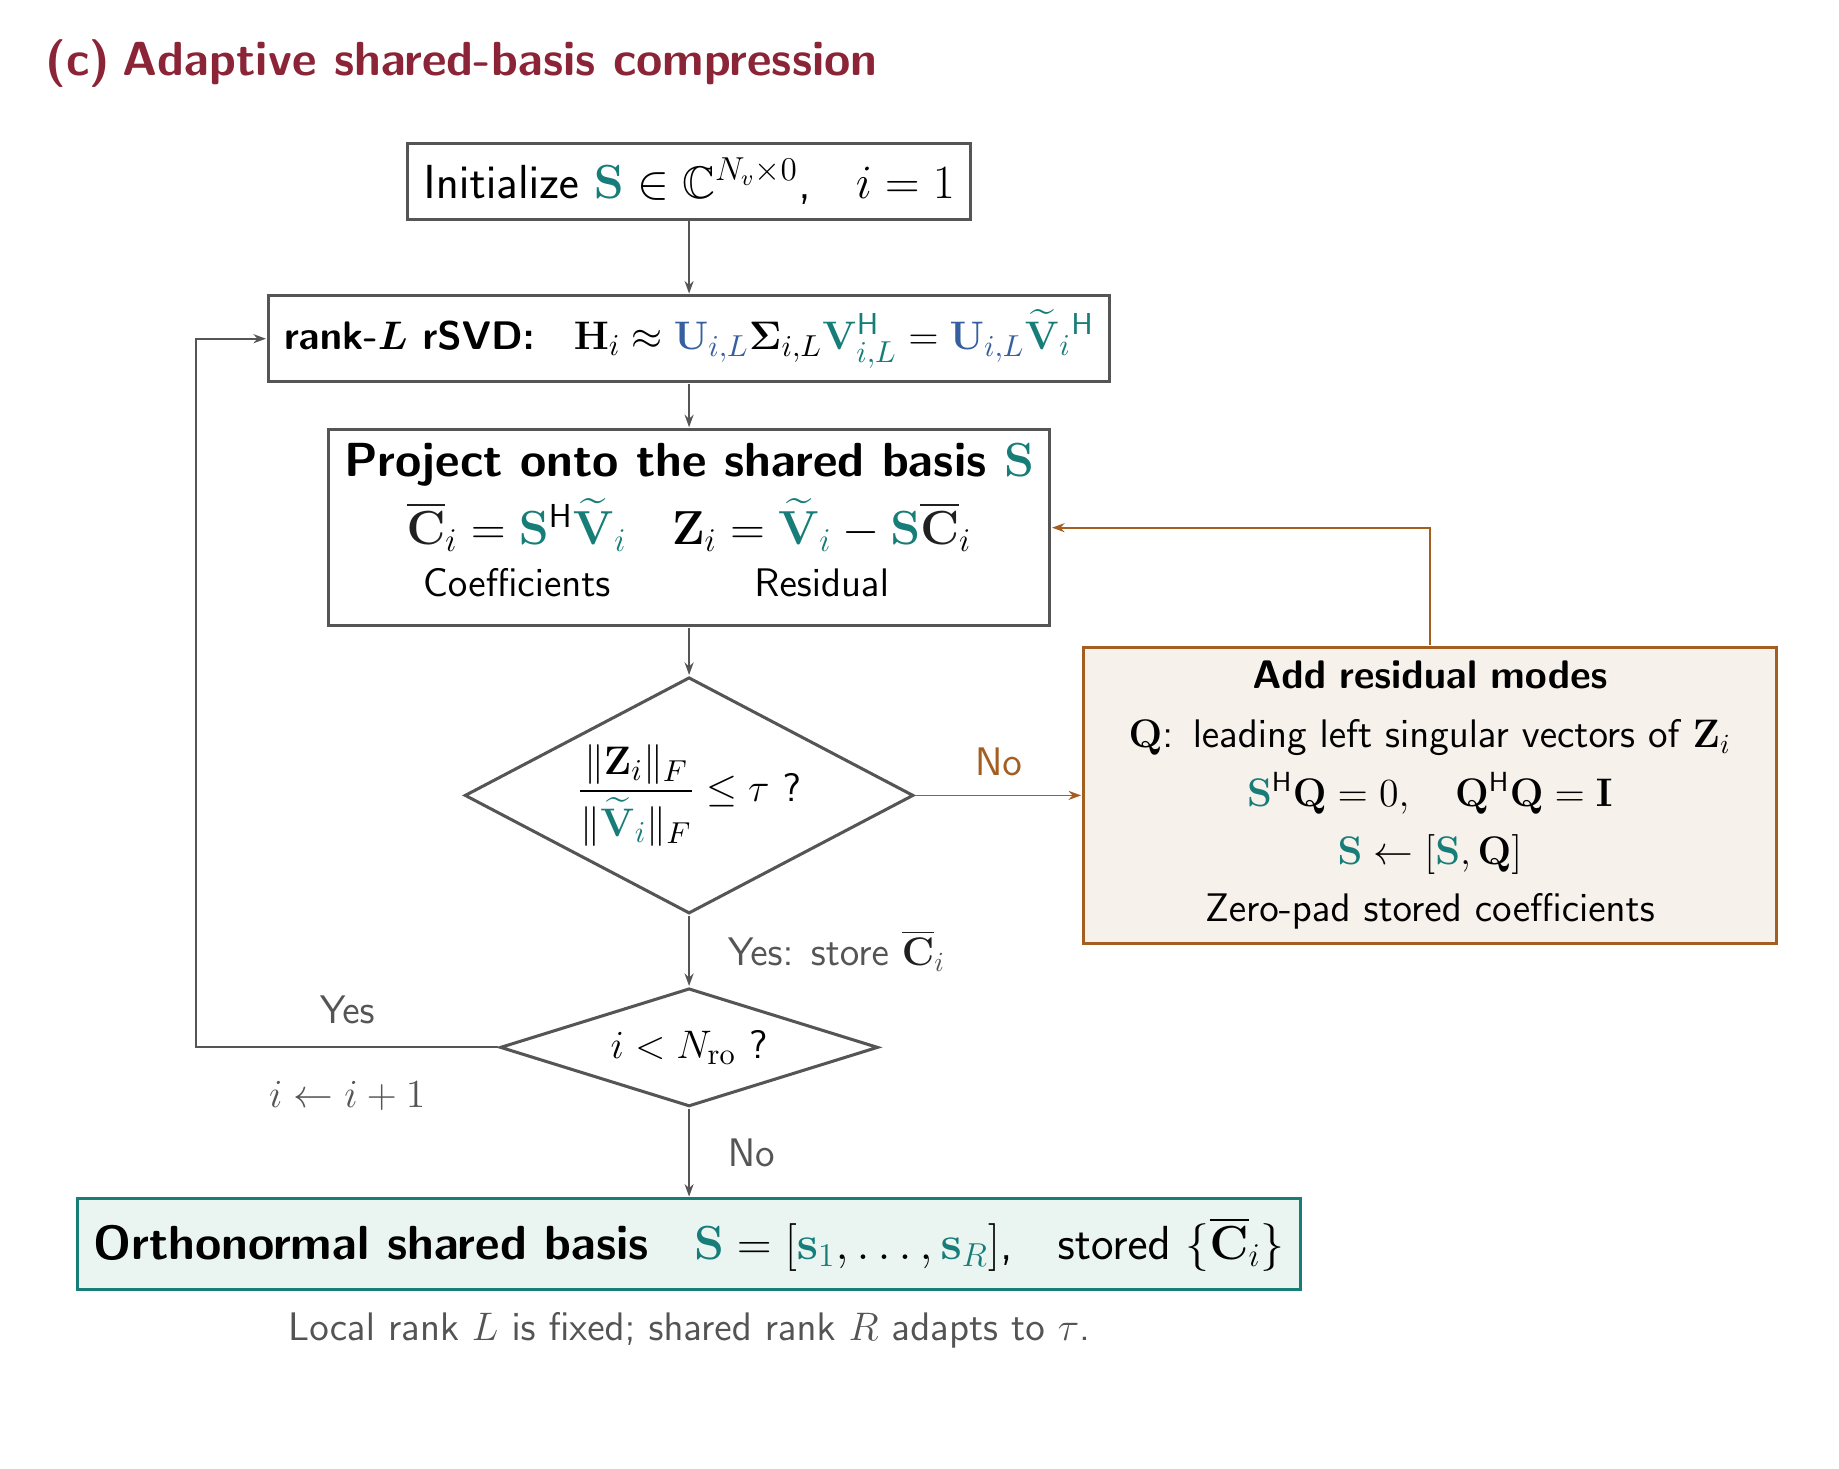
\begin{tikzpicture}[
  x=1cm,y=1cm,
  font=\fontsize{16.5}{19.5}\selectfont,
  process/.style={draw=flowgray,line width=1.1pt,rounded corners=0pt,
    fill=white,align=center,inner xsep=2mm,inner ysep=1.7mm},
  decision/.style={diamond,draw=flowgray,line width=1.1pt,fill=white,
    inner sep=0pt,align=center},
  flow/.style={figflow,draw=flowgray},
  innerloop/.style={figflow,draw=residual},
  outerloop/.style={figflow,draw=flowgray},
  link/.style={figflow,draw=ink},
  flabel/.style={font=\smalltext,text=flowgray,fill=none,inner sep=.8mm,align=center},
  encstep/.style={draw=frame,line width=.8pt,rounded corners=0pt,
    fill=wash,align=center,inner xsep=2mm,inner ysep=1.8mm},
  mathlabel/.style={font=\fontsize{15}{18}\selectfont,fill=none,align=center,inner sep=0pt}
]

\path[use as bounding box] (0,-7.25) rectangle (22.65,-25.2);
\node[draw=none,text=red,fill=none,inner sep=0pt,
    font=\bfseries\fontsize{17.307692}{20.769231}\selectfont] at (.64,-7.7) {(c)};
\node[anchor=west,text=red,fill=none,font=\bfseries\fontsize{17.307692}{20.769231}\selectfont,
    inner sep=0pt] at (1.20,-7.7) {Adaptive shared-basis compression};
% C: restore the vertical main flow and left/right nested loops.
% Show singular values explicitly, then their absorption into Vtilde.
% Keep clear connectors around the compact, single-line local-factor step.
\node[process,minimum height=.96cm] (init) at (8.4,-9.2)
  {Initialize \(\sharedbasis\in\mathbb C^{N_v\times0}\),\quad \(i=1\)};
\node[process,minimum height=1.05cm,font=\fontsize{15.5}{18.5}\selectfont] (load) at ($(init.center)+(0,-2.0)$)
  {\textbf{rank-\(\boldsymbol L\) rSVD:}\quad
    \(\mat H_i\approx{\color{timeblue}\mat U_{i,L}}\bm\Sigma_{i,L}{\color{spacegreen}\mat V_{i,L}^{\mathsf H}}
    ={\color{timeblue}\mat U_{i,L}}{\color{spacegreen}\vlocal^{\mathsf H}}\)};
\node[process,minimum height=1.6cm] (project) at ($(load.center)+(0,-2.4)$) {
  \textbf{Project onto the shared basis \(\sharedbasis\)}\\[1.3mm]
  \begin{tabular}{@{}c@{\quad}c@{}}
    \(\coef=\sharedbasis^{\mathsf H}\vlocal\) & \(\mat Z_i=\vlocal-\sharedbasis\coef\)\\[-.3mm]
    {\smalltext Coefficients} & {\smalltext Residual}
  \end{tabular}};
\node[decision,aspect=1.9,minimum width=5.7cm,minimum height=3.0cm]
  (tol) at ($(project.center)+(0,-3.4)$) {};
\node[mathlabel] (criterion) at (tol.center) {$\displaystyle
  \frac{\|\mat Z_i\|_F}{\|\vlocal\|_F}\leq\tau$ ?};
\node[process,draw=residual,fill=residual!9!white,text width=8.4cm,font=\smalltext,
  minimum height=3.6cm] (expand) at ($(tol.center)+(9.407692,0)$) {
  \textbf{Add residual modes}\\[1.3mm]
  \mbox{\(\mat Q\): leading left singular vectors of \(\mat Z_i\)}\\[1.3mm]
  \mbox{\(\sharedbasis^{\mathsf H}\mat Q=0,\quad\mat Q^{\mathsf H}\mat Q=\mat I\)}\\[1.2mm]
  \mbox{\(\sharedbasis\leftarrow[\sharedbasis,\mat Q]\)}\\[1.2mm]
  Zero-pad stored coefficients};
% Compact tolerance-to-next-readout spacing leaves room for both loop labels.
\node[decision,minimum width=4.8cm,minimum height=1.5cm] (more) at ($(tol.center)+(0,-3.2)$) {};
\node[mathlabel] at (more.center) {$i<\ro$ ?};
% Output frame is fitted to its content; its connector still uses the gutter.
\node[process,draw=spacegreen,fill=spacewash,minimum height=1.15cm]
  (shared) at ($(more.center)+(0,-2.5)$) {
  \textbf{Orthonormal shared basis}\quad \(\sharedbasis=[{\color{spacegreen}\mat s_1},\ldots,{\color{spacegreen}\mat s_R}]\),\quad
  stored \(\{\overline{\mat C}_i\}\)};

% Every execution edge is tied to node anchors; each return path has one arrowhead.
\draw[flow] (init.south) -- (load.north);
\draw[flow] (load.south) -- (project.north);
\draw[flow] (project.south) -- (tol.north);
\draw[innerloop] (tol.east) -- (expand.west);
\node[flabel,text=residual] at ($(tol.east)!0.5!(expand.west)+(0,.43)$) {No};
\coordinate (innerturn) at (expand.north |- project.east);
\draw[innerloop] (expand.north) -- (innerturn) -- (project.east);
\draw[flow] (tol.south) -- node[midway,flabel,right=4mm] {Yes: store \(\coef\)} (more.north);
\coordinate (outerrail) at ($(load.west)+(-.90,0)$);
\coordinate (outerlower) at (outerrail |- more.west);
\coordinate (outerupper) at (outerrail |- load.west);
\draw[outerloop] (more.west) -- (outerlower) -- (outerupper) -- (load.west);
\node[flabel,text=flowgray] at ($(more.west)!0.5!(outerlower)+(0,.48)$) {Yes};
\node[flabel,text=flowgray] at ($(more.west)!0.5!(outerlower)+(0,-.62)$) {$i\leftarrow i+1$};
\draw[flow] (more.south) -- node[midway,flabel,right=4mm] {No} (shared.north);
\node[text=muted,font=\smalltext,fill=none] at ($(shared.south)+(0,-.50)$)
  {Local rank \(L\) is fixed; shared rank \(R\) adapts to \(\tau\).};
% Criterion-box audit checks fraction clearance against the sloped diamond edges.
\path let \p1=(criterion.north west),\p2=(criterion.south east),
  \p3=(tol.west),\p4=(tol.east),\p5=(tol.north),\p6=(tol.south),
  \n1={abs(\x2-\x1)},\n2={abs(\y2-\y1)},
  \n3={abs(\x4-\x3)},\n4={abs(\y6-\y5)}
  in \pgfextra{\typeout{FIG1-C-CRITERION-W:\n1}
    \typeout{FIG1-C-CRITERION-H:\n2}
    \typeout{FIG1-C-CRITERION-DW:\n3}
    \typeout{FIG1-C-CRITERION-DH:\n4}};
% Build-time anchor audit, invisible in the artwork.
\foreach \anodename in {init,load,project,tol,expand,more,shared}{
  \path let \p1=(\anodename.center),\p2=(\anodename.north),\p3=(\anodename.south)
    in \pgfextra{\typeout{FIG1-C-NODE:\anodename:\x1:\y1:\y2:\y3}};
}

\end{tikzpicture}
\endgroup}
\sbox{\sharedoperatorbox}{\fontsize{7.5}{9}\selectfont$\textstyle
 \mat A_c\approx\sum_{r=1}^{R}\diag(\temporalmode)\,\mathcal F\,\diag(\spatialmode^*)\,\mat C_c$}
\sbox{\temporalweightsbox}{\fontsize{8}{9.6}\selectfont$\displaystyle
 {\color{timeblue}\widehat{\mat q}_i}={\color{timeblue}\mat U_{i,L}}\coef^{\mathsf H}$}
\sbox{\localfactorbox}{\fontsize{8}{9.6}\selectfont$\textstyle
 \mat H_i\approx{\color{timeblue}\mat U_{i,L}}{\color{spacegreen}\vlocal^{\mathsf H}}$}
\typeout{FIG1-LOCAL-FACTOR-WIDTH: \the\wd\localfactorbox}
\typeout{FIG1-SHARED-OPERATOR-WIDTH: \the\wd\sharedoperatorbox}
\typeout{FIG1-TEMPORAL-WEIGHTS-WIDTH: \the\wd\temporalweightsbox}
\typeout{FIG1-SIGNAL-WIDTH: \the\wd\signalbox}
\typeout{FIG1-C-NATIVE-WIDTH: \the\wd\compressionbox}
\null
\begin{tikzpicture}[remember picture,overlay]
\begin{scope}[shift={(current page.north west)},x=1cm,y=-1cm]
\clip (0,0) rectangle (\PageWidth,\PageHeight);
\begin{scope}[shift={(-\CropX,-\CropY)},
 font=\fontsize{8}{9.6}\selectfont,text=ink,
 head/.style={anchor=west,font=\bfseries\fontsize{9}{10.8}\selectfont,inner sep=0pt},
 small/.style={font=\fontsize{7.5}{9}\selectfont,inner sep=0pt},
 math/.style={inner sep=0pt,align=center},
 note/.style={small,text=muted,align=center},
 box/.style={draw=linegray,line width=.55pt,fill=white,align=center,inner sep=1.3mm},
 flow/.style={figflow,draw=ink}]
% (a) Physical origin; D0 and F are kept separate from the residual field H.
\ifnum\FigOneView<2
 \node[head] at (.30,.35) {(a) Signal model with static and dynamic fields};
 \node[math] at (8.75,1.21) {\usebox{\signalbox}};
 \node[math] at (1.90,1.97) {$\mat E_i=\mat D_{0,i}(\mat F_i\odot\mat H_i)$};
 \node[small,anchor=west] at (3.70,1.97) {$\mat D_{0,i}$: zeroth-order phase;\quad $\mat F_i$: Fourier encoding;\quad $\mat H_i$: $\Delta B_0$ + higher-order phase modulation};
\fi
\ifnum\FigOneView=0
 \draw[lightgray,line width=.4pt] (.30,2.42) -- (17.15,2.42);
\fi
% (b) Conceptual factorization and sharing, executed readout by readout in (c).
\ifnum\FigOneView=1\else\ifnum\FigOneView=3\else
 \node[head] at (.30,2.81) {(b) Reconstruction overview};
 % Main-axis nodes are placed from the preceding south anchor with a common gap.
 \node[small,text=muted] at (2.65,3.21) {$\Delta B_0$ + higher-order phase modulation};
 \node[anchor=north,minimum width=4.80cm,minimum height=1.42cm,inner sep=0pt,outer sep=0pt]
   (fieldmatrix) at (2.65,3.41) {};
 \begin{scope}[shift={(fieldmatrix.north)}]
   \foreach \xx/\yy in {-.69/0,-.81/.07,-.93/.14,-1.05/.21}{
     \path[draw=muted,line width=.55pt,fill=lightgray!20!white] (\xx,\yy) rectangle ++(2.10,.90);
     \foreach \dx in {.35,.70,1.05,1.40,1.75}
       \draw[linegray!60,line width=.3pt] (\xx+\dx,\yy) -- ++(0,.90);
     \foreach \dy in {.225,.45,.675}
       \draw[linegray!60,line width=.3pt] (\xx,\yy+\dy) -- ++(2.10,0);
   }
   \node[math,font=\fontsize{9}{11}\selectfont,text=ink,fill=lightgray!20!white,inner sep=.4mm] at (0,.66) {$\mat H_i$};
   \node[small,align=center,text=muted] at (-1.83,.66) {Samples\\$N_t$};
   \node[small,text=muted] at (0,1.27) {Voxels $N_v$};
   \node[small,anchor=west,text=muted] at (1.56,.66) {$i=1,\ldots,N_{\mathrm{ro}}$};
 \end{scope}
 % A single neutral outer frame holds two sequential conceptual steps.
 \node[box,anchor=north,minimum width=4.80cm,minimum height=3.60cm,inner sep=0pt]
   (compression) at ($(fieldmatrix.south)+(0,\OverviewGap)$) {};
 \begin{scope}[shift={(compression.north)}]
   \node[math,font=\bfseries\fontsize{7.5}{9}\selectfont] at (0,.38)
     {Per-readout low-rank approximation};
   % Only the spatial factor supplies the input to adaptive sharing.
   \node[math,anchor=base west,font=\fontsize{8}{9.6}\selectfont]
     (localspatial) at (.35,1.08) {$\vlocal^{\mathsf H}$};
   \node[math,anchor=base east,font=\fontsize{8}{9.6}\selectfont]
     at (localspatial.base west) {$\mat H_i\approx{\color{timeblue}\mat U_{i,L}}$};
   \draw[flow,draw=spacegreen] (localspatial.south) -- ($(localspatial.south)+(0,.27)$);
   \node[math,font=\bfseries\fontsize{7.5}{9}\selectfont,text=red] at (0,1.70)
     {Adaptive spatial-basis sharing};
   \begin{scope}[shift={(0,1.56)}]
   % Corresponding Nv, R, L dimensions retain the same displayed lengths.
   \foreach \xx/\yy in {-1.51/.40,-1.61/.45,-1.71/.50}{
     \path[draw=spacegreen!75,line width=.45pt,fill=spacewash] (\xx,\yy) rectangle ++(.44,.72);
     \draw[spacegreen!30,line width=.25pt] (\xx+.22,\yy) -- ++(0,.72);
   }
   \node[small,text=spacegreen,fill=spacewash,inner sep=.20mm] at (-1.49,.86) {$\vlocal$};
   \node[minimum width=.64cm,minimum height=.82cm,inner sep=0pt,outer sep=0pt] (localstack) at (-1.39,.81) {};
   \path[draw=spacegreen,line width=.65pt,fill=spacegreen!14!white] (-.235,.50) rectangle ++(.58,.72);
   \foreach \dx in {.19333,.38667}
     \draw[spacegreen!40,line width=.25pt] (-.235+\dx,.50) -- ++(0,.72);
   \node[minimum width=.58cm,minimum height=.72cm,inner sep=0pt,outer sep=0pt] (sharedmatrix) at (.055,.86) {};
   \node[small,text=spacegreen,fill=spacegreen!14!white,inner sep=.20mm] at (.055,.86) {$\sharedbasis$};
   \draw[flow] ($(localstack.east |- sharedmatrix.west)+(.06,0)$) -- ($(sharedmatrix.west)+(-.06,0)$);
   \node[math,text=muted] at (.78,.86) {$\times$};
   \foreach \xx/\yy in {1.29/.40,1.19/.45,1.09/.50}{
     \path[draw=linegray,line width=.45pt,fill=white] (\xx,\yy) rectangle ++(.44,.58);
     \draw[lightgray,line width=.25pt] (\xx+.22,\yy) -- ++(0,.58);
     \foreach \dy in {.19333,.38667}
       \draw[lightgray,line width=.25pt] (\xx,\yy+\dy) -- ++(.44,0);
   }
   \node[small,fill=white,inner sep=.20mm] at (1.31,.79) {$\coef$};
   \node[math] at (-1.49,1.57)
     {$\underset{\text{\fontsize{7.5}{9}\selectfont$N_v\!\times\! L$}}{{\color{spacegreen}\vlocal}}$};
   \node[math] at (-.72,1.57)
     {$\underset{\phantom{\text{\fontsize{7.5}{9}\selectfont$N_v\!\times\! L$}}}{\vphantom{\vlocal}\approx}$};
   \node[math] at (.055,1.57)
     {$\underset{\text{\fontsize{7.5}{9}\selectfont$N_v\!\times\! R$}}{\vphantom{\vlocal}{\color{spacegreen}\sharedbasis}}$};
   \node[math] at (.78,1.57)
     {$\underset{\phantom{\text{\fontsize{7.5}{9}\selectfont$N_v\!\times\! L$}}}{\vphantom{\vlocal}\times}$};
   \node[math] at (1.31,1.57)
     {$\underset{\text{\fontsize{7.5}{9}\selectfont$R\!\times\! L$}}{\vphantom{\vlocal}\coef}$};
   \end{scope}
 \end{scope}
 \draw[flow] (fieldmatrix.south) -- (compression.north);
 \node[box,anchor=north,minimum width=4.80cm,minimum height=1.90cm,inner sep=0pt]
   (weights) at ($(compression.south)+(0,\OverviewGap)$) {};
 \node[math,font=\bfseries\fontsize{7.5}{9}\selectfont] at ($(weights.north)+(0,.22)$) {Readout-specific temporal factors};
 \node[math] at ($(weights.north)+(0,.70)$) {\usebox{\temporalweightsbox}};
 \node[note] at ($(weights.north)+(0,1.20)$) {Apply zeroth-order phase};
 \node[note] at ($(weights.north)+(0,1.54)$) {Concatenate readouts $\rightarrow{\color{timeblue}\mat q}$};
 \draw[flow] (compression.south) -- (weights.north);
 \node[box,anchor=north,minimum width=4.80cm,minimum height=2.25cm,inner sep=0pt]
   (encoding) at ($(weights.south)+(0,\OverviewGap)$) {};
 \node[math,font=\bfseries\fontsize{7.5}{9}\selectfont] at ($(encoding.north)+(0,.22)$) {Shared encoding operator};
 \node[math] at ($(encoding.north)+(0,.72)$) {\usebox{\sharedoperatorbox}};
 \node[note] at ($(encoding.north)+(0,1.40)$) {$\temporalmode,\spatialmode$: temporal and spatial factors\\of shared mode $r$};
 \node[note] (nufftcalls) at ($(encoding.north)+(0,2.00)$)
   {NUFFT calls per coil: $\ro L\rightarrow{\color{spacegreen}R}$};
 \draw[flow] (weights.south) -- (encoding.north);
 \node[box,anchor=north,minimum width=2.85cm,minimum height=.55cm,inner sep=0pt,
   font=\bfseries\fontsize{7.5}{9}\selectfont]
   (recon) at ($(encoding.south)+(0,\OverviewGap)$) {CG reconstruction};
 \draw[flow] (encoding.south) -- (recon.north);
 % Build-time layout audit; these markers add no visible content.
 \foreach \anodename in {fieldmatrix,compression,weights,encoding,recon}{
   \path let \p1=(\anodename.center),\p2=(\anodename.north),\p3=(\anodename.south)
     in \pgfextra{\typeout{FIG1-B-NODE:\anodename:\x1:\y1:\y2:\y3}};
 }
 \foreach \aprev/\anext in {fieldmatrix/compression,compression/weights,weights/encoding,encoding/recon}{
   \path let \p1=(\aprev.south),\p2=(\anext.north),\n1={abs(\y1-\y2)}
     in \pgfextra{\typeout{FIG1-B-GAP:\aprev/\anext:\n1}};
 }
\fi\fi
% A grouping brace, with no arrowhead, identifies the entire module detailed in (c).
\ifnum\FigOneView=0
 \draw[draw=red,line width=.45pt,decorate,
   decoration={brace,amplitude=1.1mm}]
   ($(compression.north east)+(.06,0)$) -- ($(compression.south east)+(.06,0)$);
 \node[small,text=red,align=center,anchor=west] (detailnote)
   at ($(compression.east)+(.38,0)$) {Zoom-in\\(c)};
\fi
% (c) Complete nested-loop algorithm; weighted spatial-factor definition is in the caption.
\ifnum\FigOneView=1\else\ifnum\FigOneView=2\else
 \node[anchor=north west,inner sep=0pt] at (5.45,2.58) {\scalebox{.52}{\usebox{\compressionbox}}};
 \begin{scope}[shift={(6.75,12.25)}]
   \node[anchor=base west,font=\bfseries\fontsize{8.5}{10}\selectfont,inner sep=0pt] (notationtitle) at (0,0) {Notation};
   % Both columns are left aligned; every symbol-description gap is 1.5 mm.
   \node[small,anchor=base west] (notationindices) at (0,.42) {$i,c$:\hspace{1.5mm}readout / receive-coil indices};
   \node[small,anchor=base west] (notationimage) at (0,.76) {$m(\mat r)$:\hspace{1.5mm}complex image};
   \node[small,anchor=base west] (notationcoil) at (0,1.10) {$C_c(\mat r)$:\hspace{1.5mm}coil sensitivity};
   \node[small,anchor=base west] (notationterms) at (4.90,.42) {$\mathcal H$:\hspace{1.5mm}modeled higher-order term indices};
   \node[small,anchor=base west] (notationreadouts) at (4.90,.76) {$N_{\mathrm{ro}}$:\hspace{1.5mm}number of readouts};
   \node[small,anchor=base west] (notationnorm) at (4.90,1.10) {$\|\cdot\|_F$:\hspace{1.5mm}Frobenius norm};
   \node[small,anchor=base west] (notationadjoint) at (4.90,1.44) {$(\cdot)^{\mathsf H}$:\hspace{1.5mm}Hermitian transpose};
   \node[small,anchor=base west] (notationtolerance) at (0,1.78) {$\tau$:\hspace{1.5mm}relative spatial-factor error tolerance};
   \node[small,anchor=base west] (notationfourier) at (0,1.44) {$\mathcal F$:\hspace{1.5mm}stacked Fourier encoding};
   % Content-fitted background only; it cannot become an algorithm node or cover text.
   \begin{pgfonlayer}{background}
     \node[fit=(notationtitle)(notationindices)(notationimage)(notationcoil)
       (notationterms)(notationreadouts)(notationnorm)(notationadjoint)
       (notationtolerance)(notationfourier),fill=notationwash,draw=none,
       rounded corners=0pt,inner sep=1.75mm] (notationbackground) {};
   \end{pgfonlayer}
 \end{scope}

\fi\fi
\end{scope}
\end{scope}
\end{tikzpicture}
\end{document}
